\documentclass[12pt]{article}
\usepackage[utf8]{inputenc}
\usepackage[margin=0.9in]{geometry}
\usepackage{paralist}
\usepackage{blindtext}
\usepackage{hyperref}
\usepackage{chngcntr}
\usepackage{amsfonts,latexsym,amsthm,amssymb,amsmath,amscd,euscript}
\usepackage{enumitem}
\usepackage{caption}
\usepackage{algorithm}
\usepackage{algpseudocode}
\usepackage{amsmath}
\usepackage[table,xcdraw]{xcolor}
\usepackage{tikz}
\usepackage{parskip}
\usepackage{fancyhdr}


    \hypersetup{colorlinks=true,citecolor=blue,urlcolor =black,linkbordercolor={1 0 0}}

\usetikzlibrary{calc}

\renewcommand\thesubsubsection{\arabic{subsubsection}}

\newenvironment{statement}{\color[rgb]{1.00,0.00,0.50} {}}{}


\newcolumntype{M}[1]{>{\centering\arraybackslash}m{#1}}
\newcolumntype{N}{@{}m{0pt}@{}}
\algnewcommand{\algorithmicand}{\textbf{ and }}


\algnewcommand\algorithmicforeach{\textbf{for each}}
\algdef{S}[FOR]{ForEach}[1]{\algorithmicforeach\ #1\ \algorithmicdo}


\newlist{enums}{enumerate}{3}

\setlist[enums, 1]{label={(\arabic*)}, noitemsep}
\setlist[enums, 2]{label={-}, noitemsep}

\hypersetup{
    colorlinks=true,
    linkcolor=blue,
    filecolor=magenta,
    urlcolor=black
    }

\title{ADA Assignment 1}
% \author{Anirudh S. Kumar (2021517), Aakarsh Jain (2021507)}
\author{
    \\\vspace{0em} Anirudh S. Kumar \\\vspace{-0.5em}
    \footnotesize{Roll Number - 2021517}\\\vspace{-0.5em}
    \footnotesize{IIIT - Delhi}\\\vspace{-0.5em}
    \footnotesize{\href{mailto:anirudh21517@iiitd.ac.in}{\texttt{anirudh21517@iiitd.ac.in}}}
  \and
    \\\vspace{0em} Vartika\\\vspace{-0.5em}
    \footnotesize{Roll Number - 2021571}\\\vspace{-0.5em}
    \footnotesize{IIIT - Delhi}\\\vspace{-0.5em}
    \footnotesize{\href{mailto:vartika21571@iiitd.ac.in}{\texttt{vartika21571@iiitd.ac.in}}}
    \vspace{1em}
}

\renewcommand{\footrulewidth}{0.4pt}% Default \footrulewidth is 0pt
\renewcommand{\headrulewidth}{0pt}% Default \headrulewidth is 0.4pt


\date{\today}

\begin{document}
\maketitle

\pagestyle{fancy}
\fancyhf{}
\fancyfoot[L]{Anirudh S. Kumar}
\fancyfoot[R]{Vartika}

\section{L Shaped Tiles}
\subsection{Problem}
\begin{statement}
    Consider the problem of putting L-shaped tiles (L-shaped consisting of three squares)
    in an \texttt{n × n} square-board. You can assume that \texttt{n} is a power of 2. Suppose that one square of this
    board is defective and tiles cannot be put in that square. Also, two L-shaped tiles cannot intersect
    each other. Describe an algorithm that computes a proper tiling of the board. Justify the running
    time of your algorithm.
\end{statement}


\subsection{Proof}

\subsubsection{Pre Processing}

Iterate through the board and find which cell is the defective cell. Time complexity for this process is $\mathcal{O}(n^2)$ where $n \times n$ is the size of the board

\subsubsection{Base Case: \texttt{n = 2} i.e. it's a \texorpdfstring{$2 \times 2$}{Lg} board }

\begin{table}[ht]
    \centering
    \begin{tabular}{|M{20pt}|M{20pt}|N}
        \hline
          &                          \\[20pt]
        \hline
          & \cellcolor[HTML]{FE0000} \\[20pt]
        \hline
    \end{tabular}
\end{table}

One square is defective. We can place one L shaped tile in the remaining space.

\subsubsection{Sub Problem}

\begin{enums}[label={(\arabic*)}, noitemsep]
    \item Divide the board into 4 boards of size $n/2 \times n/2$ each
    \item Check which board out of these 4 has the defective tile
    \item Of the 3 sub boards which don't have a defective tile, assume there is an L shaped tile between them like shown in the figure.
    \item Recursively apply the algorithm for all the boards now. We can assume that the positions which already have a piece of tile as defective.
\end{enums}

\begin{table}[!htbp]
    \centering
    \begin{tabular}{|M{20pt}|M{20pt}|M{20pt}|M{20pt}|N}
        \hline
          &                          &   &   \\[20pt]\hline
          & \cellcolor[HTML]{FE0000} &   &   \\[20pt] \hline
          &                          &   &   \\[20pt] \hline
          &                          &   &   \\[20pt] \hline
    \end{tabular}
    \vspace{2pt}
    \begin{tabular}{|M{20pt}|M{20pt}|M{20pt}|M{20pt}|N}
        \hline
                                 &   &   &   \\[20pt]\hline
                                 &   &   &   \\[20pt] \hline
                                 &   &   &   \\[20pt] \hline
        \cellcolor[HTML]{34FF34} &   &   &   \\[20pt] \hline
    \end{tabular}

    \begin{tabular}{|M{20pt}|M{20pt}|M{20pt}|M{20pt}|N}
        \hline
          &   &   & \cellcolor[HTML]{34FF34} \\[20pt]\hline
          &   &   &                          \\[20pt] \hline
          &   &   &                          \\[20pt] \hline
          &   &   &                          \\[20pt] \hline
    \end{tabular}
    \begin{tabular}{|M{20pt}|M{20pt}|M{20pt}|M{20pt}|N}
        \hline
        \cellcolor[HTML]{34FF34} &   &   &   \\[20pt]\hline
                                 &   &   &   \\[20pt] \hline
                                 &   &   &   \\[20pt] \hline
                                 &   &   &   \\[20pt] \hline
    \end{tabular}
\end{table}
\subsubsection{How to combine solution}
Place an L shaped tile in the location we assumed in (3) in Sub Problem.
\subsubsection{Recursive Algorithm}

% \begin{algorithm}

\begin{algorithm}
    \begin{algorithmic}[1]

        \Ensure $board \leftarrow int[n][n]$
        \Require {defective $\leftarrow$ the defective cell}
        \If{$n = 2$}
        \State Place a L shaped tile on the board
        \Else


        \State {Find which quadrant the defective cell belongs to}
        \State {Place an L shaped tile at the common corner of the other 3 quadrants}
        \State {Mark these cells as defective}
        \State {Run the algorithm for all the quadrants}
        \EndIf
    \end{algorithmic}
\end{algorithm}

\pagebreak

\subsubsection{Time complexity}

We need to find the defective tile for every board of size \texttt{n x n}, which will take $n^2$ comparisons.

In the Divide Step, we break each problem into 4 problems of size $n^2/4$ each. Therefore, we will get the following recurrence relation for $T(n^2)$





$$T(n^2) = 4T(n^2/4) + c$$
Let $n^2 = k$, where $k$ is the number of tiles on the board, then our recurrence relation in $T(k)$ now becomes

$$T(k) = 4T(k/4) + c$$


Looking at this equation, we can see that it can easily be solved using Master's Theorem for $a = 4$, $b = 4$ and $d = 0$
Since $d < \log_b(a)$, we will get time tome complexity as  :-

$$\mathcal{O}(k^{\log_b{a}}) = \mathcal{O}(k) = \mathcal{O}(n^2)$$

Therefore, final time complexity of the algorithm comes out to be $$\mathcal{O}(n^2 + \mathcal{O}(n^2)) = \mathcal{O}(n^2) $$
{\qed}



\pagebreak

\section{Largest Subset of L}

\subsection{Problem}

\begin{statement}
    Suppose we are given a set $L$ of $n$ line segments in 2D plane. Each line segment has
    one endpoint on the line $y = 0$, one endpoint on the line $y = 1$ and all the $2n$ points are distinct.
    Give an algorithm that uses dynamic programming and computes a largest subset of $L$ of which
    every pair of segments intersects each other. You must also give a justification why your algorithm
    works correctly.
\end{statement}

\begin{center}


    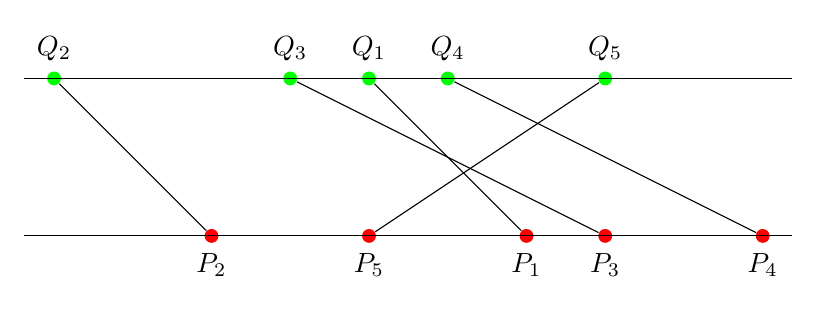
\begin{tikzpicture}[dot/.style={circle,inner sep=1pt,fill,label={#1},name=#1},
            extended line/.style={shorten >=-#1,shorten <=-#1},
        extended line/.default=1cm]

        \node at (1,1) (A){};
        \node at (10,1) (B) {};
        \node at (1,3) (C) {};
        \node at (10, 3) (D) {};

        \node [dot=below:$P_1$, fill=red, minimum size=5pt] at (7, 1) (p1) {};
        \node [dot=above:$Q_1$, fill=green, minimum size=5pt] at (5, 3) (q1) {};
        \node [dot=below:$P_2$, fill=red, minimum size=5pt] at (3, 1) (p2) {};
        \node [dot=above:$Q_2$, fill=green, minimum size=5pt] at (1, 3) (q2) {};
        \node [dot=below:$P_3$, fill=red, minimum size=5pt] at (8, 1) (p3) {};
        \node [dot=above:$Q_3$, fill=green, minimum size=5pt] at (4, 3) (q3) {};
        \node [dot=below:$P_4$, fill=red, minimum size=5pt] at (10, 1) (p4) {};
        \node [dot=above:$Q_4$, fill=green, minimum size=5pt] at (6, 3) (q4) {};
        \node [dot=below:$P_5$, fill=red, minimum size=5pt] at (5, 1) (p5) {};
        \node [dot=above:$Q_5$, fill=green, minimum size=5pt] at (8, 3) (q5) {};

        \draw [extended line=0.5cm] (A) -- (B);
        \draw [extended line=0.5cm] (C) -- (D);
        \draw (p1) -- (q1);
        \draw (p2) -- (q2);
        \draw (p3) -- (q3);
        \draw (p4) -- (q4);
        \draw (p5) -- (q5);

    \end{tikzpicture}

\end{center}

\subsection{Proof}

\subsubsection{Pre Processing}

Let $L = [\{x_1, x_2\}]_n$ be the list of line segments where $x_1$ is the coordinate of the point at $y = 0$, and $x_2$ is the coordinate of the point at $y = 1$.

Sort the given list of line segments w.r.t $x_1$ in decreasing order, and construct a list \\ $a[i] = [x_2$ for $\{x_1, x_2\}$ in $L]$


\subsubsection{Sub Problem}

$d[i]$ stores the length of the largest increasing subsequence upto and including $a[i]$.

Initialize $d[i] = 1$ $\forall i \in \{0, 1, 2, \dots n\}$.
Our task is now to find $d[i]$ given we know all $d[j], j < i$


\subsubsection{Recurrence Relation}


If $d[i] = 1$, then it's the only element in the subsequence, but if $d[i] > 1$, then $\exists j < i$, a[$j$] $<$ a[$i$] such that $d[j] = d[i] - 1$ i.e. There must be some subsequence of length $d[i] - 1$ which ends at a[$j$]


Converting the above statement into a recurrence relation, we get the following recurrence relation of $d[i]$

\[
    d[i] =  \max \left(
    1,
    \max_{\substack{j < i, \\
        \text{a[$j$] $<$ a[$i$]}}}
    (d[j] + 1)
    \right)
\]

\subsubsection{Sub Problem that solves the original problem}
The solution to the problem will be $\max(d[i])$, and then find the actual subsequence corresponding to the index with maximum $d[i]$ value.

To achieve this, we will use an auxilary array $p$, which will store the $j$ value we have discussed above, i.e., the $j$ for which $d[i]$ is maximum.

Once we have reached the end of the algorithm and found $i$ for which $d[i]$ is maximum, we will backtrack using this auxilary array to find the subsequence, and hence our subset.

\subsubsection{Algorithm}

\begin{algorithm}
    % \caption{}\label{alg:p2}
    \begin{algorithmic}[1]
        \Require a $\leftarrow$ int[n]
        \Require L $\leftarrow$ int[n][2] \Comment{Array of line segments in sorted order}


        \State $d \leftarrow$ int[n]
        \State $d[i] = 1$ $\forall i$
        \State $p \leftarrow$ int[n]
        \State $p[i] = -1$ $\forall i$

        \For {$i$ in range(0, n)} \Comment{Calculating $d$ and $p$}
        \For {$j$ in range (0, i)}
        \If {$a[j] < a[i]$}
        \State $d[i] = d[j] + 1$
        \State $p[i] = j$
        \EndIf
        \EndFor
        \EndFor

        \State idx $\leftarrow$ 0
        \State val $\leftarrow$ $d[0]$
        \For {$i$ in range(0, n)}   \Comment{Finding the maximum value of i}
        \If {$d[i] >$ val}
        \State val $\leftarrow d[i]$
        \State idx $\leftarrow i$
        \EndIf
        \EndFor

        \State set $\leftarrow \{\}$ \Comment{making a set to add all line segments into}

        \While {idx $\neq -1$}
        \State set.add(L[idx])
        \State idx $\leftarrow$ $p$[idx]

        \EndWhile

        \Return set
    \end{algorithmic}
\end{algorithm}


\subsubsection{Proof of Correctness}

For any pair of lines $P_1(x_1, x_2), Q_1(x_3, x_4)$, where $x_1, x_3$ are the $x$-coordinates on $y = 0$ and $x_2, x_4$ are the $x$-coordinates on $y = 1$, they will only intersect if $(x_1 - x_3) \dot (x_2 - x_4) < 0$. In our case, we ensure that $x_1 - x_3 > 0$ by sorting the list of line segments in decreasing order.

Therefore, we only need to check for all pairs $(x_2, x_4)$ such that $x_2 < x_4$. In any increasing sequence $x_1, x_2, \dots x_k$, all the pair will mutually intersect.

This reduces our problem to finding the Longest Increasing Subsequence in an array where the line segmemnts are sorted in decreasing order by their point on $y = 0$


\subsubsection{Time Complexity}

We can observe that for every $i$, we must check all $j < i$ to find the maximum $d[j]$. This will take $\mathcal{O}(n)$ number of operations for every $i$

Since we are performing this opertation for every $i$, therefore our final time complexiy comes out to be $\mathcal{O}(n^2)$
\qed












\pagebreak

\subsection{\texorpdfstring{$\mathcal{O}(n\log(n))$}{Lg} approach}

\subsubsection{Pre Processing}

Let $L = [\{x_1, x_2\}]_n$ be the list of line segments where $x_1$ is the coordinate of the point at $y = 0$, and $x_2$ is the coordinate of the point at $y = 1$.

Sort the given list of line segments w.r.t $x_1$ in decreasing order, and construct a list \\ $a[i] = [x_2$ for $\{x_1, x_2\}$ in $L]$


\subsubsection{Sub-problem}

$dp[i]$ stores smallest element for which an increasing subsequence of length $i$ exists. For example, for the array ${[6, 4, 5, 7, 1]}$,
$dp[i] = [-\infty, 1, 5, 7, \infty, \dots]$

Here, $\infty$ signifies that there isn't a increasing subsequence of length $i$

\subsubsection{Base Case}

$dp[i] = \infty $ $\forall i \in \{1, 2, 3, \dots n\}$ where n is total number of segments, and $dp[0] = -\infty$

\subsubsection{Sub-problem which solves the original problem}

The value of $i$ for which $dp[i]$ is the largest finite number in the array will give us the length of the longest increasing subsequence. Remember that $i$ gives us the length of the LIS and $dp[i]$ is the value at which the LIS of length $i$ ends.


\subsubsection{Algorithm}

\begin{algorithm}
    \begin{algorithmic}[1]
        \Require L $\leftarrow$ int[n][2] \Comment{Array of line segments in sorted order}
        \Require a $\leftarrow$ int[n] \Comment{The same $a$ mentioned in pre processing}
        \State $d \leftarrow$ int[n+1]
        \State $d[0] = -\infty$
        \State $d[i] = \infty$ $\forall i > 0$

        \For {i in range(0, n)}
        \State $l \leftarrow$ smallest value of $l$ such that $d[l] > a[i]$
        \If {$d[l-1] < a[i]$ \and $a[i] < d[l]$}
        \State $d[l] \leftarrow a[i]$
        \EndIf

        \EndFor

        \State ans $\leftarrow 0$
        \For {$i$ in range(0, n+1)}
        \If {$d[i] = \infty$}
        \State \textbf{break}
        \EndIf

        \State ans $\leftarrow d[i]$
        \EndFor
    \end{algorithmic}
\end{algorithm}

\subsubsection{Proof of Correctness}

For any pair of lines $P_1(x_1, x_2), Q_1(x_3, x_4)$, where $x_1, x_3$ are the $x$-coordinates on $y = 0$ and $x_2, x_4$ are the $x$-coordinates on $y = 1$, they will only intersect if $(x_1 - x_3) \dot (x_2 - x_4) < 0$. In our case, we ensure that $x_1 - x_3 > 0$ by sorting the list of line segments in decreasing order.

Therefore, we only need to check for all pairs $(x_2, x_4)$ such that $x_2 < x_4$. In any increasing sequence $x_1, x_2, \dots x_k$, all the pair will mutually intersect.

This reduces our problem to finding the Longest Increasing Subsequence in an array where the line segmemnts are sorted in decreasing order by their point on $y = 0$



\subsubsection{Time Complexity}

Time complexity of sorting the array during preprocessing is $\mathcal{O}(n\log(n))$

For finding the value of $l$ as shows in (5) of the algorithm, we notice that $d$ is always a non decreasing subarray. Therefore to find $l$ such that $d[l] > a[i]$, we can use binary search. Time complexity of the binary search comes out to be $\mathcal{O}(\log(n))$

We iterating over the length of $a$ and performing binary search $\forall i$. Therefore, final complexity of the algorithm comes out to be $\mathcal{O}(n\log(n))$
\qed

\pagebreak

\section{Shipments}

\subsection{Problem}

\begin{statement}
    Suppose that an equipment manufacturing company manufactures $s_i$ units in the
    $i^{th}$ week. Each week’s production has to be shipped by the end of that week. Every week, one of the
    three shipping agents A, B and C are involved in shipping that week’s production and they charge
    in the following:
    \begin{itemize}
        \item Company A charges $a$ rupees per unit.
        \item  Company B charges $b$ rupees per week (irrespective of the number of units), but will only ship for a block of 3 consecutive weeks.
        \item Company C charges $c$ rupees per unit but returns a reward of $d$ rupees per week, but will
              not ship for a block of more than 2 consecutive weeks. It means that if $s_i$ unit is shipped in
              the $i^{th}$ week through company C, then the cost for $i^{th}$ week will be $c s_i - d$.
    \end{itemize}
    The total cost of the schedule is the total cost to be paid to the agents. If $s_i$ unit is produced in the
    $i^{th}$ week, then $s_i$ unit has to be shipped in the $i^{th}$ week. Then, give an efficient algorithm that
    computes a schedule of minimum cost.
\end{statement}


\subsection{Proof}

\subsubsection{Sub Problem}

$dp[i]$ is the optimal cost till $i$th week without considering company $C$ , and $dp'[i]$ is the optimal cost till the $i^{th}$ week considering $C$


\subsubsection{Recurrence Relation}

For the $0^{th}$ week, no products have been shipped, therefore
$dp[0] = dp'[0] = 0$.

We can't use $B$ for shipping until we know number of weeks $>$ 2. Therefore,
For the first week,
cost of shipping by $A$ is
$$dp[1] = a s_1$$
Minimum cost of shipping using either $A$ or $C$ is minimum of shipping cost by $A$ and shipping cost by $C$
\begin{align*}
    dp'[1] = \min \Biggl(
    \begin{array}{cc}
    dp[1],                \\
    c s_1 - d
    \end{array}
    \Biggr)
\end{align*}


For the second week,
Minimum cost of shipping by $A$ is minimum cost till last week $+$ cost shipping by $A$ in second week is
$$dp[2] = dp'[1] + a s_2$$

Minimum of cost of shipping by either $A$ or $C$ is $\mathbf{min}$(cost of shipping by $A$ in week 2,  cost of shipping till week 1 $+$ cost of shipping by $C$ in week 2, cost of shipping by $C$ in two consecutive weeks \textit{i.e.} shipping by $C$ in present week and in last week)


$$dp'[2] = \min
\Biggl(
\begin{array}{cc}
    dp[2],                      \\
    dp[1] + c s_2 - d,          \\
    dp[0] + c (s_2 + s_1) - 2 d
\end{array}
\Biggr)
$$
From third week onwards,
Cost of shipping by $A$ will change slightly as now we can ship using $B$ also.
Therefore, while calculating $A$ we will also take care of cost of shipping by $B$ in 3 consecutive weeks.

$$dp[i] = \min
\Biggl(
\begin{array}{c}
    dp'[i-1] + a s_i, \\
    dp'[i-3] + 3b
\end{array}
\Biggr)
$$

Calculation of $dp'$ will remain same

$$dp'[i] = \min
\Biggl(
\begin{array}{c}
    dp[i],                           \\
    dp[i-1] + cs_i - d,              \\
    dp[i-2] + c(s_i + s_{i-1}) - 2 d
\end{array}
\Biggr)
$$

\subsubsection{Sub Problem that will solve the original problem}

$dp'[n]$ will give us the minimum cost of shipping over $n$ weeks

\subsubsection{Algorithm}

\begin{algorithm}
    \begin{algorithmic}
        \Require a $\leftarrow$ int \Comment{ Cost of shipping of company A per unit}

        \Require b $\leftarrow$ int \Comment{ Cost of shipping of company B per week}

        \Require c $\leftarrow$ int \Comment{ Cost of shipping of company C per unit}

        \Require d $\leftarrow$ int \Comment{Reward per week on shipping by company C}

        \Require s $\leftarrow$ int[n] \Comment{number of items to be shipped in $i^{th}$ week}

        \State $dp \leftarrow$ int[n]
        \State $dp' \leftarrow$ int[n]


        \State $dp[0] = dp'[0] = 0$.
        \State $dp[1] = a s_1$
        \State $dp'[1] = \min(c s_1 - d, dp[1])$
        \State $dp[2] = dp'[1] + a s_2$
        \State $dp'[2] = \min(dp[2], dp[1] + c s_2 - d, dp[0] + c(s_2 + s_1) - 2 d)$

        \For {i in range(3, n)}
        \State $dp[i] = \min(dp'[i-1] + a s_i, dp'[i-3] + 3b)$
        \State $dp'[i] = \min(dp[i], dp[i-1] + c s_i - d, dp[i-2] + c(s_i + s_{i-1}) - 2 d)$

        \EndFor

        \Return $dp'[n]$



    \end{algorithmic}
\end{algorithm}

\pagebreak

\subsubsection{Time Complexity}

As we are iterating through the array only once, this means that the time complexity of our algorithm is $\mathcal{O}(n)$ where $n$ is the number of weeks.


\section{Acknowledgements}

\begin{itemize}
    \item Dev Mittal - 2021038 for Q3
    \item \href{https://cp-algorithms.com/sequences/longest_increasing_subsequence.html#solution-in-on-log-n-with-dynamic-programming-and-binary-search}{CP-Algorithms} for Question 2 $\mathcal{O}(n\log(n))$ solution
\end{itemize}



\end{document}
